\newpage

\section{Experimento 3} 
En este experimento se busca visualizar mediante el osciloscopio la interferencia de la red eléctrica que es generada por el acoplamiento inductivo que se propaga a través de los cables. 
Para ello se conectó un cable a la punta del osciloscopio con una longitud similar al cable conectado al negativo de  la misma punta, generando un circuito abierto. Luego se colocó entre medio de los dos cables el cable de alimentación del osciloscopio que está conectado a la red eléctrica.
\begin{figure}[H]
    \centering
    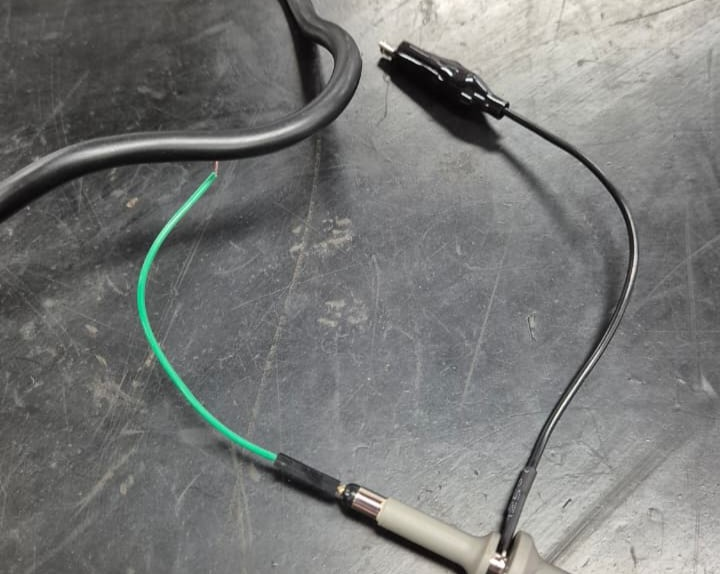
\includegraphics[width=0.5\textwidth]{images/exp3.jpeg}
    \caption{Implementación utilizada para medir la interferencia.}
    \label{fig:experimento3}
\end{figure}
Una vez configurado el osciloscopio para medir la señal acoplada de 50Hz, se observó lo siguiente:
\begin{figure} [H]
    \centering
    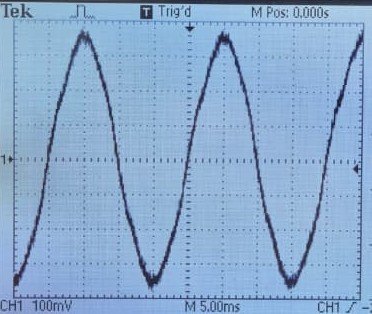
\includegraphics[width=0.5\textwidth]{images/50hz3.jpeg}
    \caption{Señal acoplada de 50Hz.}
    \label{fig:experimento3_result}
\end{figure}
Valores medido de la señal acoplada de 50Hz:
\begin{itemize}
    \item Amplitud: $756mV_{pp}$
    \item Frecuencia: $49,85Hz\simeq 50Hz$
    \item$V_{RMS}: 267mV$
\end{itemize}